%%%% Paramétrage du TD %%%%
\def\xxactivite{ \ifprof \normalsize{TD 6 -- Corrigé } \else  \ifcolle Colle \else TD 6\fi \fi} % \normalsize \vspace{-.4cm}
\def\xxauteur{\textsl{Xavier Pessoles}}

\def\xxnumchapitre{Chapitre 2 \vspace{.2cm}}
\def\xxchapitre{\hspace{.12cm} Hyperstatisme}



\def\xxcompetences{%
\vspace{-.5cm}
\footnotesize{
\textsl{%
\textbf{Savoirs et compétences :}\\
\vspace{-.2cm}
\begin{itemize}[label=\ding{112},font=\color{ocre}] 
%\item \textit{Mod2.C34} : chaînes de solides;
\item \textit{Mod2.C34} : degré de mobilité du modèle;
\item \textit{Mod2.C34} : degré d’hyperstatisme du modèle;
\item \textit{Mod2.C34.SF1} : déterminer les conditions géométriques associées à l’hyperstatisme;
\item \textit{Mod2.C34} : résoudre le système associé à la fermeture cinématique et en déduire le degré de mobilité et d’hyperstatisme.
\end{itemize}}}}

\def\xxtitreexo{Robovolc}
\def\xxsourceexo{\hspace{.2cm} \footnotesize{X ENS -- PSI 2017}}

\def\xxfigures{
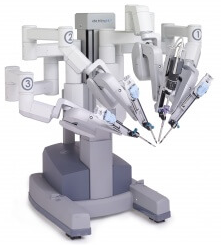
\includegraphics[width=.75\textwidth]{fig_00}
}%figues de la page de garde




\pagestyle{empty}


%%%%%%%% PAGE DE GARDE COURS
\ifcours
\begin{tikzpicture}[remember picture,overlay]
\node at (current page.north west)
{\begin{tikzpicture}[remember picture,overlay]
\node[anchor=north west,inner sep=0pt] at (0,0) {\includegraphics[width=\paperwidth]{\thechapterimage}};
\draw[anchor=west] (-2cm,-8cm) node [line width=2pt,rounded corners=15pt,draw=ocre,fill=white,fill opacity=0.6,inner sep=40pt]{\strut\makebox[22cm]{}};
\draw[anchor=west] (1cm,-8cm) node {\huge\sffamily\bfseries\color{black} %
\begin{minipage}{1cm}
\rotatebox{90}{\LARGE\sffamily\textsc{\color{ocre}\textbf{\xxnumpartie}}}
\end{minipage} \hfill
\begin{minipage}[c]{14cm}
\begin{titrepartie}
\begin{flushright}
\renewcommand{\baselinestretch}{1.1} 
\Large\sffamily\textsc{\textbf{\xxpartie}}
\renewcommand{\baselinestretch}{1} 
\end{flushright}
\end{titrepartie}
\end{minipage} \hfill
\begin{minipage}[c]{3.5cm}
{\large\sffamily\textsc{\textbf{\color{ocre} \discipline}}}
\end{minipage} 
 };
\end{tikzpicture}};
\end{tikzpicture}


\begin{tikzpicture}[overlay]
\node[shape=rectangle, 
      rounded corners = .25 cm,
	  draw= ocre,
	  line width=2pt, 
	  fill = ocre!10,
	  minimum width  = 2.5cm,
	  minimum height = 3cm,] at (18cm,0) {};
\node at (17.7cm,0) {\rotatebox{90}{\textbf{\Large\color{ocre}{\classe}}}};
%{};
\end{tikzpicture}

\vspace{3.5cm}

\begin{tikzpicture}[remember picture,overlay]
\draw[anchor=west] (-2cm,-6cm) node {\huge\sffamily\bfseries\color{black} %
\begin{minipage}{2cm}
\begin{center}
\LARGE\sffamily\textsc{\color{ocre}\textbf{\xxactivite}}
\end{center}
\end{minipage} \hfill
\begin{minipage}[c]{15cm}
\begin{titrechapitre}
\renewcommand{\baselinestretch}{1.1} 
\Large\sffamily\textsc{\textbf{\xxnumchapitre}}

\Large\sffamily\textsc{\textbf{\xxchapitre}}
\vspace{.5cm}

\renewcommand{\baselinestretch}{1} 
\normalsize\normalfont
\xxcompetences
\end{titrechapitre}
\end{minipage}  };
\end{tikzpicture}
\vfill

\begin{flushright}
\begin{minipage}[c]{.3\linewidth}
\begin{center}
\xxfigures
\end{center}
\end{minipage}\hfill
\begin{minipage}[c]{.6\linewidth}
\startcontents
\printcontents{}{1}{}
\end{minipage}
\end{flushright}

\begin{tikzpicture}[remember picture,overlay]
\draw[anchor=west] (4.5cm,-.7cm) node {
\begin{minipage}[c]{.2\linewidth}
\begin{flushright}

\includegraphics[width=2cm]{png/logoCC}
\end{flushright}
\end{minipage}
\begin{minipage}[c]{.2\linewidth}
\textsl{\xxauteur} \\
\textsl{\classe}
\end{minipage}
 };
\end{tikzpicture}
\newpage
\pagestyle{fancy}

\newpage
\pagestyle{fancy}

\else
\fi


%%%%%%%% PAGE DE GARDE TD
\iftd
%\begin{tikzpicture}[remember picture,overlay]
%\node at (current page.north west)
%{\begin{tikzpicture}[remember picture,overlay]
%\draw[anchor=west] (-2cm,-3.25cm) node [line width=2pt,rounded corners=15pt,draw=ocre,fill=white,fill opacity=0.6,inner sep=40pt]{\strut\makebox[22cm]{}};
%\draw[anchor=west] (1cm,-3.25cm) node {\huge\sffamily\bfseries\color{black} %
%\begin{minipage}{1cm}
%\rotatebox{90}{\LARGE\sffamily\textsc{\color{ocre}\textbf{\xxnumpartie}}}
%\end{minipage} \hfill
%\begin{minipage}[c]{13.5cm}
%\begin{titrepartie}
%\begin{flushright}
%\renewcommand{\baselinestretch}{1.1} 
%\Large\sffamily\textsc{\textbf{\xxpartie}}
%\renewcommand{\baselinestretch}{1} 
%\end{flushright}
%\end{titrepartie}
%\end{minipage} \hfill
%\begin{minipage}[c]{3.5cm}
%{\large\sffamily\textsc{\textbf{\color{ocre} \discipline}}}
%\end{minipage} 
% };
%\end{tikzpicture}};
%\end{tikzpicture}

%%%%%%%%%% PAGE DE GARDE TD %%%%%%%%%%%%%%%
%\begin{tikzpicture}[overlay]
%\node[shape=rectangle, 
%      rounded corners = .25 cm,
%	  draw= ocre,
%	  line width=2pt, 
%	  fill = ocre!10,
%	  minimum width  = 2.5cm,
%	  minimum height = 2.5cm,] at (18.5cm,0) {};
%\node at (17.7cm,0) {\rotatebox{90}{\textbf{\Large\color{ocre}{\classe}}}};
%%{};
%\end{tikzpicture}

% PARTIE ET CHAPITRE
%\begin{tikzpicture}[remember picture,overlay]
%\draw[anchor=west] (-1cm,-2.1cm) node {\large\sffamily\bfseries\color{black} %
%\begin{minipage}[c]{15cm}
%\begin{flushleft}
%\xxnumchapitre \\
%\xxchapitre
%\end{flushleft}
%\end{minipage}  };
%\end{tikzpicture}

% Bandeau titre exo
\begin{tikzpicture}[remember picture,overlay]
\draw[anchor=west] (-2cm,-4cm) node {\huge\sffamily\bfseries\color{black} %
\begin{minipage}{5cm}
\begin{center}
\LARGE\sffamily\color{ocre}\textbf{\textsc{\xxactivite}}

\begin{center}
\xxfigures
\end{center}

\end{center}
\end{minipage} \hfill
\begin{minipage}[c]{12cm}
\begin{titrechapitre}
\renewcommand{\baselinestretch}{1.1} 
\large\sffamily\textbf{\textsc{\xxtitreexo}}

\small\sffamily{\textbf{\textit{\color{black!70}\xxsourceexo}}}
\vspace{.5cm}

\renewcommand{\baselinestretch}{1} 
\normalsize\normalfont
\xxcompetences
\end{titrechapitre}
\end{minipage}  };
\end{tikzpicture}

\else
\fi


%%%%%%%% PAGE DE GARDE FICHE
\iffiche
\begin{tikzpicture}[remember picture,overlay]
\node at (current page.north west)
{\begin{tikzpicture}[remember picture,overlay]
\draw[anchor=west] (-2cm,-3.25cm) node [line width=2pt,rounded corners=15pt,draw=ocre,fill=white,fill opacity=0.6,inner sep=40pt]{\strut\makebox[22cm]{}};
\draw[anchor=west] (1cm,-3.25cm) node {\huge\sffamily\bfseries\color{black} %
\begin{minipage}{1cm}
\rotatebox{90}{\LARGE\sffamily\textsc{\color{ocre}\textbf{\xxnumpartie}}}
\end{minipage} \hfill
\begin{minipage}[c]{14cm}
\begin{titrepartie}
\begin{flushright}
\renewcommand{\baselinestretch}{1.1} 
\large\sffamily\textsc{\textbf{\xxpartie} \\} 

\vspace{.2cm}

\normalsize\sffamily\textsc{\textbf{\xxnumchapitre -- \xxchapitre}}
\renewcommand{\baselinestretch}{1} 
\end{flushright}
\end{titrepartie}
\end{minipage} \hfill
\begin{minipage}[c]{3.5cm}
{\large\sffamily\textsc{\textbf{\color{ocre} \discipline}}}
\end{minipage} 
 };
\end{tikzpicture}};
\end{tikzpicture}


\begin{tikzpicture}[overlay]
\node[shape=rectangle, 
      rounded corners = .25 cm,
	  draw= ocre,
	  line width=2pt, 
	  fill = ocre!10,
	  minimum width  = 2.5cm,
	  minimum height = 2.5cm,] at (18.5cm,0.5cm) {};
%	  minimum height = 2.5cm,] at (18.5cm,0cm) {};
\node at (17.7cm,0.5) {\rotatebox{90}{\textsf{\textbf{\large\color{ocre}{\classe}}}}};
%{};
\end{tikzpicture}



\else
\fi




\setlength{\columnseprule}{.1pt}

\pagestyle{fancy}
\thispagestyle{plain}

\ifprof
\vspace{5cm}
\else
\vspace{5cm}
\fi

\def\columnseprulecolor{\color{ocre}}
\setlength{\columnseprule}{0.4pt} 

%%%%%%%%%%%%%%%%%%%%%%%

\setcounter{exo}{0}



%\ifprof
%\else
\begin{multicols}{2}
%\fi
\section*{Mise en situation}





\begin{obj}
Dans cette sous-partie, on établit un modèle statique du châssis de ROBOVOLC.
\end{obj}

La mobilité sur terrain accidenté est obtenue, en plus de par la motorisation indépendante des
roues, par l'utilisation d'un châssis articulé. Celui-ci a une structure tubulaire avec des articulations
passives (non actionnées) permettant à ROBOVOLC de s'adapter à toute surface non plane. Une
illustration des cinq mouvements indépendants permis par les articulations est donnée sur la
\autoref{fig_11}.

\begin{figure}[H]
\centering
\begin{tabular}{|p{.45\linewidth}|p{.45\linewidth}|}
\hline
Châssis au repos & Mouvement 1 : rotation de l'essieu avant
autour de l'axe longitudinal  \\ \hline
\begin{center}
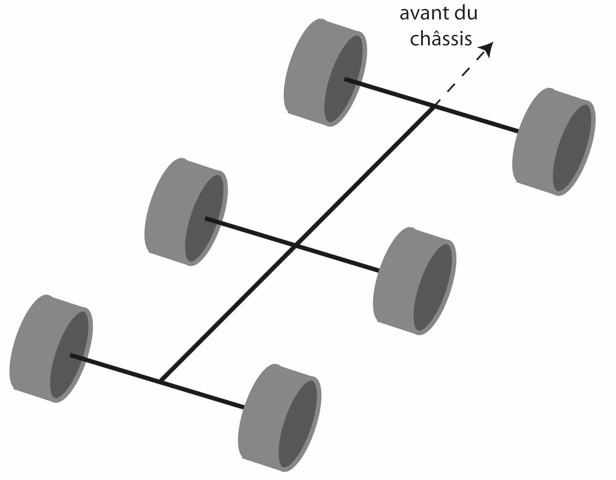
\includegraphics[width=.9\linewidth]{fig_11_a.png}
\end{center}
&
\begin{center}
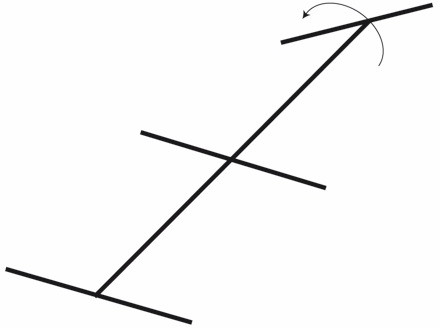
\includegraphics[width=.9\linewidth]{fig_11_b.png}
\end{center}
\\ \hline
Mouvement 2 :
rotation de l'essieu central
autour de l'axe longitudinal & Mouvement 3 :
rotation de l'essieu arrière
autour de l'axe longitudinal  \\ \hline
\begin{center}
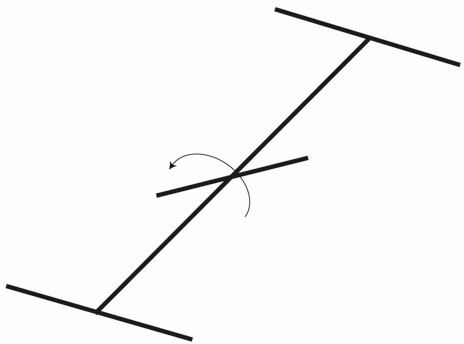
\includegraphics[width=.9\linewidth]{fig_11_c.png}
\end{center} 
& 
\begin{center}
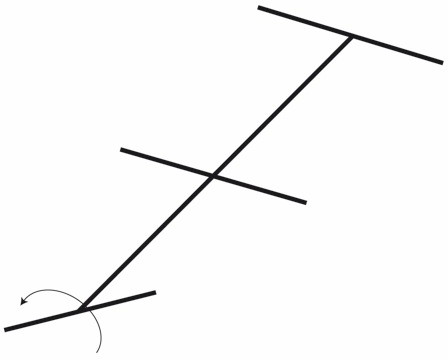
\includegraphics[width=.9\linewidth]{fig_11_d.png}
\end{center} \\ \hline
Mouvement 4 :
rotation de l'arbre avant
autour de l'axe transversal &
Mouvement 5 :
rotation de l'arbre arrière
autour de l'axe transversal \\ \hline
\begin{center}
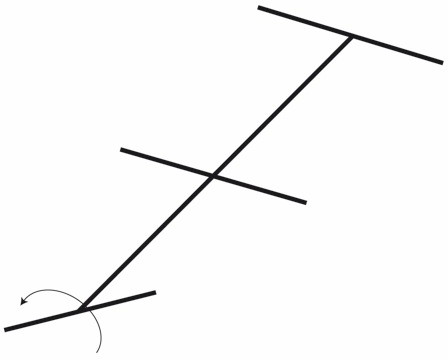
\includegraphics[width=.9\linewidth]{fig_11_e.png}
\end{center}
&
\begin{center}
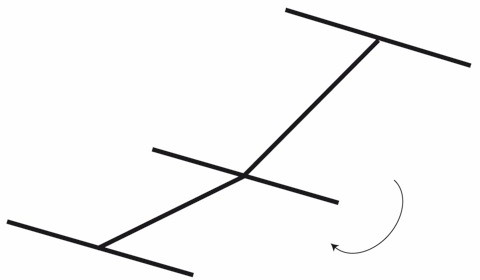
\includegraphics[width=.9\linewidth]{fig_11_f.png}
\end{center} \\ \hline
\end{tabular}

\caption{Illustration des mouvements de déformation du châssis\label{fig_11}}
\end{figure}

Le châssis est composé de cinq parties orientables les unes par rapport aux autres (\autoref{fig_12}) :
\begin{itemize}
\item l'essieu avant, noté EAV, reliant les roues avant 1 et 2 ;
\item l'essieu central, noté EC, reliant les roues centrales 3 et 4 ;
\item l'essieu arrière, noté EAR, reliant les roues arrière 5 et 6 ;
\item l'arbre avant, noté AAV, connectant les essieux EAV et EC ;
\item l'arbre arrière, noté AAR, connectant les essieux EC et EAR.
\end{itemize}
On rappelle que l'empattement entre deux essieux successifs est noté $a$, et que la distance entre
deux roues d'un même essieu est notée $2e$.
Les différentes parties sont reliées entre elles par des articulations possédant une raideur en
rotation imposée. Par la suite, on supposera cette raideur négligeable devant les autres actions
mécaniques mises en jeu.
Un schéma cinématique de la plateforme (châssis+roues) est présenté sur la \autoref{fig_12}.

\begin{figure}[H]
\centering
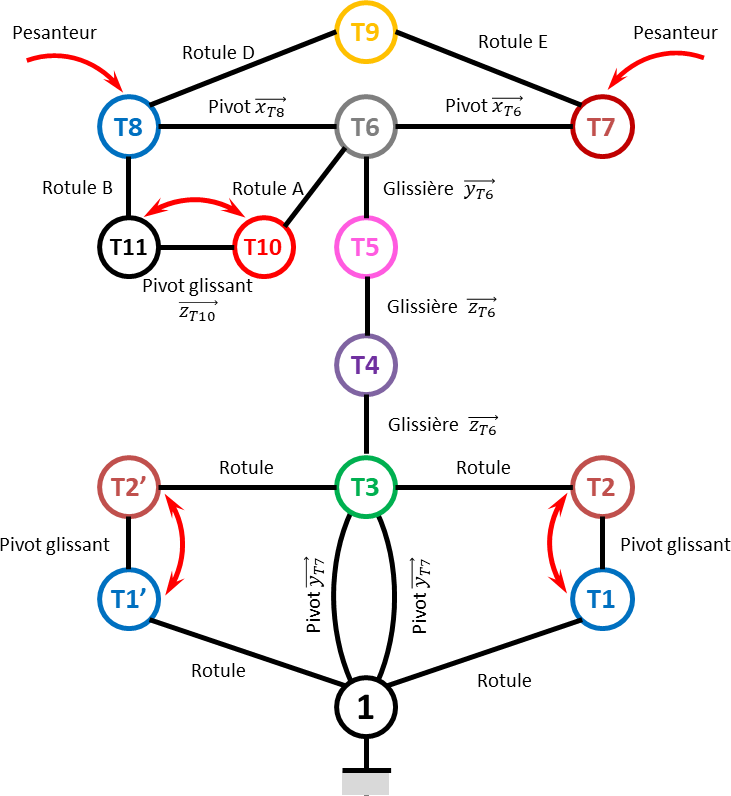
\includegraphics[width=8cm]{fig_12.png}
\caption{Schéma cinématique de la plateforme\label{fig_12}}
\end{figure}

Les deux articulations EC-AAV et EC-AAR, situées à une distance longitudinale $\pm b$ de l'essieu
EC, autorisent une rotation selon les directions $\vect{x}$ et $\vect{y}$; elles sont modélisées par des liaisons
rotule à doigt de centres respectifs $B$ et $C$. Les deux articulations EAV-AAV et EAR-AAR
autorisent une rotation selon la direction $\vect{x}$ seulement ; elles sont modélisées par des liaisons
pivot d'axe $\axe{O}{x}$.

D'autre part, les six liaisons essieu-roue sont modélisées par des liaisons pivot d'axe $\axe{A}{y}$
(roues avant), $\axe{O}{y}$ (roues centrales) ou $\axe{D}{y}$ (roues arrière). De plus, le contact de chaque
roue i avec le sol est modélisé en première approche par une liaison ponctuelle de normale
$\axe{P_i}{z}$.

On considère dans les questions \ref{q3.1} et \ref{q3.2} que les liaisons sont parfaites sans frottements.


\question{ \label{q3.1} Déterminer le nombre de mobilités du modèle du système.}

\question{ \label{q3.2} Montrer que le modèle est isostatique. Conclure quant à la capacité du châssis à maintenir
les roues au contact du sol en toute circonstance.}

\question{ \label{q3.3} Proposer un modèle de liaison parfaite pour le contact roue-sol qui permet de tenir compte,
dans une étude de statique sans glissement, du frottement longitudinal et transversal. Peut-on
calculer toutes les inconnues statiques de liaison dans ce cas ?}




\end{multicols}
